\documentclass[UTF8,fontset=fandol,11pt]{ctexart}

\usepackage[a4paper,margin=2.2cm]{geometry}
\usepackage{graphicx}
\usepackage{booktabs}
\usepackage{longtable}
\usepackage{tabularx}
\usepackage{array}
\usepackage{xcolor}
\usepackage{hyperref}
\usepackage{enumitem}
\usepackage{seqsplit}
\usepackage{tikz}
\usetikzlibrary{arrows.meta,positioning,shapes.geometric}

\graphicspath{{figures/}}

\definecolor{Accent}{HTML}{0F6B5B}
\definecolor{Soft}{HTML}{F2F8F6}
\definecolor{Line}{HTML}{D9E4E0}
\definecolor{Ink}{HTML}{182622}
\definecolor{Muted}{HTML}{5F6F6A}

\hypersetup{
  colorlinks=true,
  linkcolor=Accent,
  urlcolor=Accent,
  citecolor=Accent
}

\setlength{\parindent}{0pt}
\setlength{\parskip}{0.62em}
\setlist[itemize]{leftmargin=1.6em,itemsep=0.2em,topsep=0.2em}
\setlist[enumerate]{leftmargin=1.8em,itemsep=0.25em,topsep=0.2em}
\renewcommand{\arraystretch}{1.25}

\newcommand{\code}[1]{\texttt{\small\seqsplit{#1}}}
\newcommand{\tagbox}[2]{%
  \fcolorbox{Line}{Soft}{\begin{minipage}[t]{0.18\linewidth}\textcolor{Muted}{\small #1}\\[-0.1em]\textbf{#2}\end{minipage}}%
}

\title{\textbf{Nasri 2016 论文复现功能展示与说明}\\
\large 两阶段论文拆解与大模型多轮协作工作台}
\author{论文复现 Demo：\code{nasri\_2016\_ac\_uc\_benders}}
\date{2026 年 5 月}

\begin{document}
\maketitle

\begin{abstract}
本文档用于展示 \code{nasri\_2016\_ac\_uc\_benders} 版本的论文复现 demo。当前页面把复现流程拆成两个阶段：阶段一负责从论文中抽取复现条件，阶段二负责通过大模型多轮对话推进数据补全、脚本生成、功能修复和结果展示。文档同时给出工具链说明、页面截图和第二阶段多轮对话生成本地文件的具体实例，便于在 Overleaf 上与同伴协作修改。
\end{abstract}

\section{页面整体效果}

页面顶部已经从大面积指标卡改成轻量状态标签，只保留展示时真正需要解释的状态：论文拆解、数据表、待确认项、图表和当前复现角色。

\begin{figure}[htbp]
  \centering
  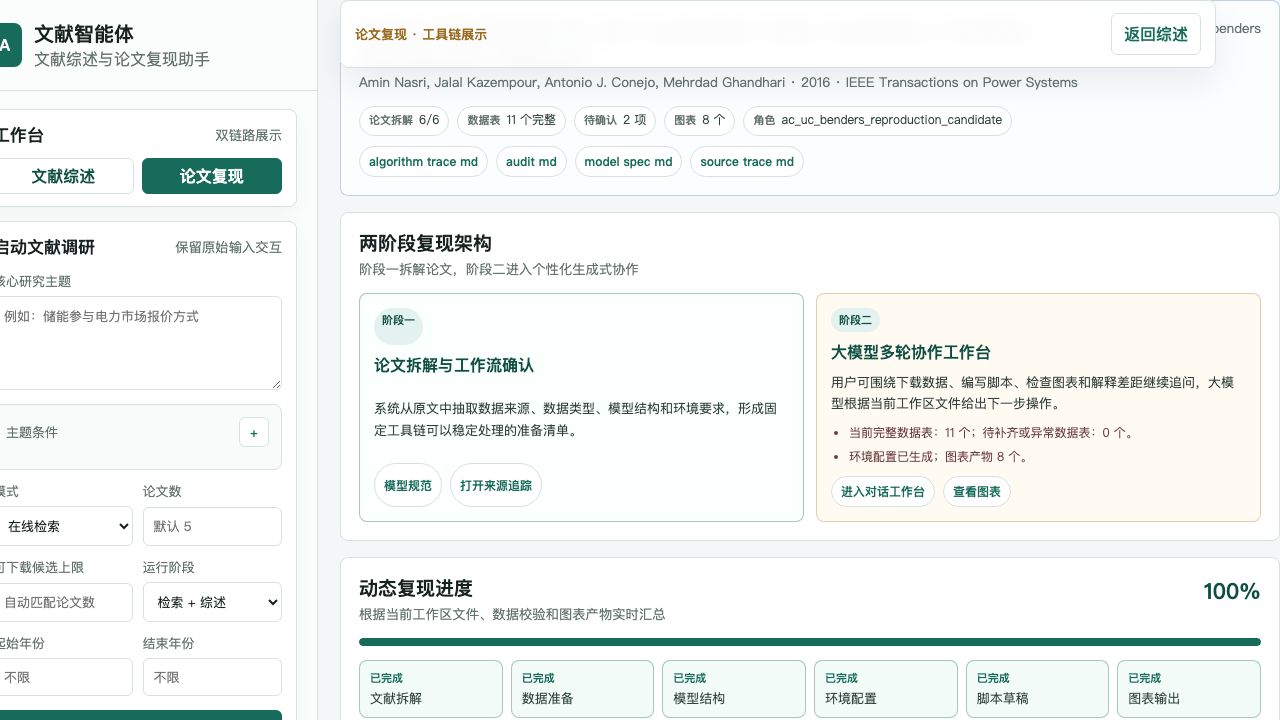
\includegraphics[width=\linewidth]{showcase_clean_header.png}
  \caption{论文复现页面顶部的清爽摘要区}
  \label{fig:clean-header}
\end{figure}

展示时可以说明：

\begin{itemize}
  \item 当前目标论文为 Nasri et al. 2016 的不确定性 AC unit commitment 论文。
  \item 阶段一已经完成论文拆解，并形成数据、模型、环境和结果展示材料。
  \item 当前工作区已有 11 个完整数据表、8 个关键图表，剩余 2 个待确认项主要是可选假设或边界表。
\end{itemize}

\section{两阶段功能结构}

\subsection{阶段一：论文拆解}

阶段一的目标是把论文复现条件整理成固定、可检查的工程输入。该阶段不强调开放式聊天，而是强调稳定抽取：

\begin{itemize}
  \item 数据来源：原文表格、公开 RTS/MATPOWER、原文图形替代构造。
  \item 模型结构：集合、变量、目标函数、约束、不确定性描述。
  \item 环境配置：求解器配置、实验矩阵、复现假设。
  \item 工作流：转录表格、生成数据、校验数据、运行模型、渲染图表。
\end{itemize}

\subsection{阶段二：多轮对话与生成式工作台}

阶段二面向用户的个性化需求。用户可以围绕“还缺什么数据”“如何写脚本”“图表为什么有差距”“哪些文件要放入上下文”继续追问。页面把数据、参数、处理产物和对话生成产物合并到一个工作文件缓存区。

\begin{figure}[htbp]
  \centering
  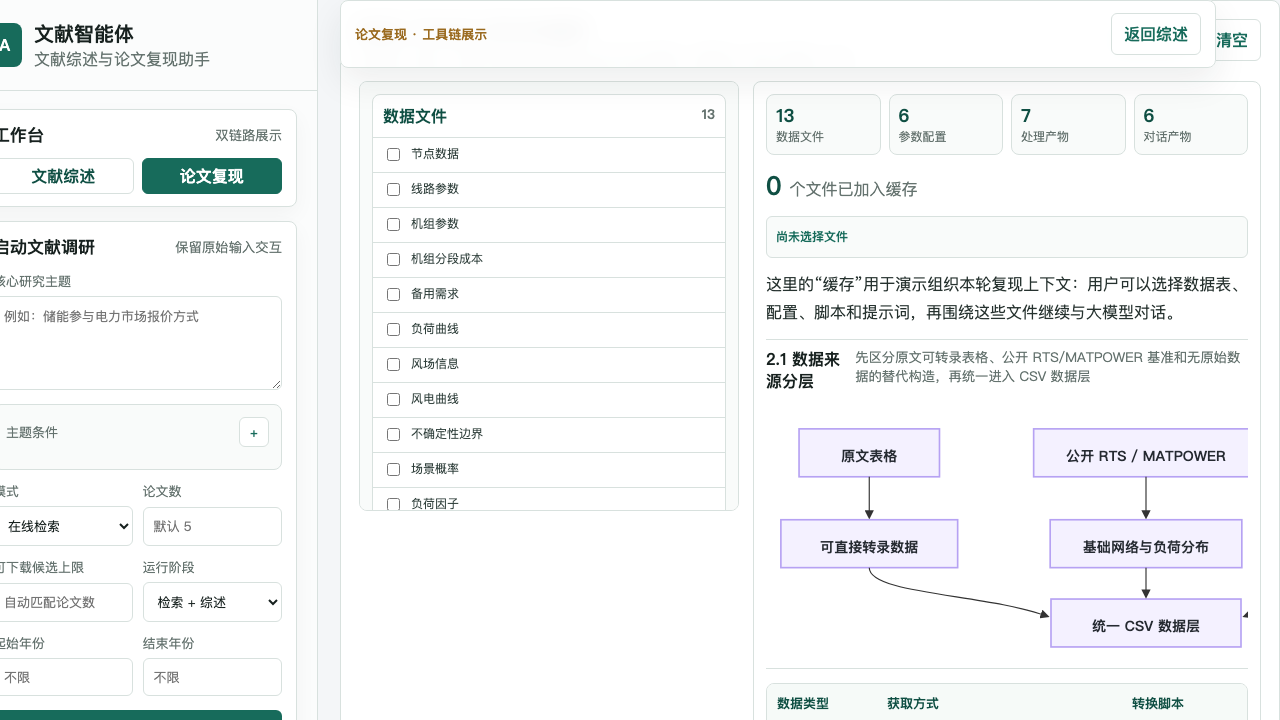
\includegraphics[width=\linewidth]{showcase_stage_two_cache.png}
  \caption{阶段二产出与工作文件缓存区}
  \label{fig:stage-two-cache}
\end{figure}

这里的设计重点是：文件不再以材料清单的方式堆在页面上，而是作为阶段二多轮对话的上下文来源。用户可以选择需要的 CSV、配置、脚本或提示词，再让大模型基于这些文件继续生成下一步。

\section{数据来源分层}

Nasri 论文的数据来源并不是单一渠道。当前版本用“来源分层 + 转换脚本”的方式展示数据如何进入统一 CSV 层。

\begin{center}
\begin{tikzpicture}[
  node distance=1.4cm and 1.55cm,
  source/.style={draw=Accent!45,fill=Accent!6,rounded corners=2pt,minimum width=3.0cm,minimum height=0.82cm,align=center,font=\small},
  merge/.style={draw=Accent!65,fill=Accent!9,rounded corners=2pt,minimum width=3.2cm,minimum height=0.82cm,align=center,font=\small\bfseries},
  arrow/.style={-Latex,thick,draw=Ink!75}
]
\node[source] (paper) {原文表格};
\node[source,right=of paper] (rts) {公开 RTS / MATPOWER};
\node[source,right=of rts] (fig) {原文图形但无原始数据};
\node[source,below=of paper] (trans) {可直接转录数据};
\node[source,below=of rts] (base) {基础网络与负荷分布};
\node[source,below=of fig] (synthetic) {合成替代数据};
\node[merge,below=1.45cm of base] (csv) {统一 CSV 数据层};
\draw[arrow] (paper) -- (trans);
\draw[arrow] (rts) -- (base);
\draw[arrow] (fig) -- (synthetic);
\draw[arrow] (trans) to[bend right=12] (csv);
\draw[arrow] (base) -- (csv);
\draw[arrow] (synthetic) to[bend left=12] (csv);
\end{tikzpicture}
\end{center}

\begin{longtable}{p{0.18\linewidth}p{0.28\linewidth}p{0.25\linewidth}p{0.21\linewidth}}
\toprule
\textbf{来源层} & \textbf{内容} & \textbf{处理方式} & \textbf{结果}\\
\midrule
\endhead
原文表格 & Table I--IV 中的线路、机组、负荷因子和场景概率 & \code{transcribe\_nasri\_tables.py} & 生成线路、机组、负荷因子和场景概率 CSV\\
公开 RTS/MATPOWER & \code{case24\_ieee\_rts.m} 中的基础网络与负荷分布 & \code{fill\_bus\_load\_fractions.py} & 将 Pd/Qd 与 24 小时负荷因子合成负荷曲线\\
原文图形但无原始数据 & Fig. 3 风电场景曲线 & \code{generate\_surrogate\_wind\_profiles.py} & 生成 40 场景 $\times$ 24 小时 $\times$ 2 风场的替代风电时序\\
案例调整 & 原文实验设定和已转录表格 & \code{apply\_nasri\_case\_adjustments.py} & 统一写入 \code{data/} 下的 CSV 数据层\\
\bottomrule
\end{longtable}

展示时需要强调：合成替代数据不会被包装成论文原始数据，而是明确标记为可审查、可替换的复现假设。

\section{工具链说明}

当前工具链可以概括为以下链路：

\begin{center}
\begin{tikzpicture}[
  node distance=0.95cm,
  workflowstep/.style={draw=Line,fill=Soft,rounded corners=2pt,minimum width=6.8cm,minimum height=0.72cm,align=center,font=\small},
  arrow/.style={-Latex,thick,draw=Accent!70}
]
\node[workflowstep] (a) {论文 PDF / target.yaml};
\node[workflowstep,below=of a] (b) {正文与证据片段抽取};
\node[workflowstep,below=of b] (c) {LLM 审计与模型结构抽取};
\node[workflowstep,below=of c] (d) {复现目录与数据模板};
\node[workflowstep,below=of d] (e) {数据转录与替代构造脚本};
\node[workflowstep,below=of e] (f) {数据校验};
\node[workflowstep,below=of f] (g) {模型求解与中间结果};
\node[workflowstep,below=of g] (h) {论文风格图表与展示页面};
\node[workflowstep,below=of h] (i) {阶段二多轮对话产物};
\foreach \x/\y in {a/b,b/c,c/d,d/e,e/f,f/g,g/h,h/i} \draw[arrow] (\x) -- (\y);
\end{tikzpicture}
\end{center}

\begin{longtable}{p{0.22\linewidth}p{0.34\linewidth}p{0.34\linewidth}}
\toprule
\textbf{模块} & \textbf{文件或目录} & \textbf{作用}\\
\midrule
\endhead
论文元信息 & \code{target.yaml} & 记录论文标题、作者、年份、目标角色\\
文本证据 & \code{extracted\_text/} & 保存 PDF 文本和证据片段\\
模型抽取 & \code{artifacts/model\_spec.json}、\code{artifacts/model\_spec.md} & 把论文模型整理成实现清单\\
数据层 & \code{data/*.csv} & 统一复现输入数据\\
数据校验 & \code{reports/data\_validation.json} & 汇总完整、空表、缺失和可选空表\\
数据构造脚本 & \code{src/transcribe\_nasri\_tables.py} 等 & 将原文、公开基准和替代构造写入 CSV\\
复现结果 & \code{results/} & 保存求解结果、图表数据和对比结果\\
阶段二产物 & \code{dialogue\_outputs/} & 保存多轮对话生成的候选数据、脚本和说明\\
\bottomrule
\end{longtable}

\section{第二阶段多轮对话的具体作用}

\subsection{示例需求}

在展示中点击“运行示例对话”，模拟用户提出如下需求：

\begin{quote}
请基于当前待补齐或待确认数据表，生成一轮面向本论文的数据补全、功能修复和效果展示方案。
\end{quote}

系统会读取当前 Nasri 工作区状态：正式数据表已经可运行，但 \code{reserves.csv} 和 \code{uncertainty\_bounds.csv} 属于可选或待确认材料。多轮对话并不是泛泛回答，而是生成可以落到本地的文件。

\begin{figure}[htbp]
  \centering
  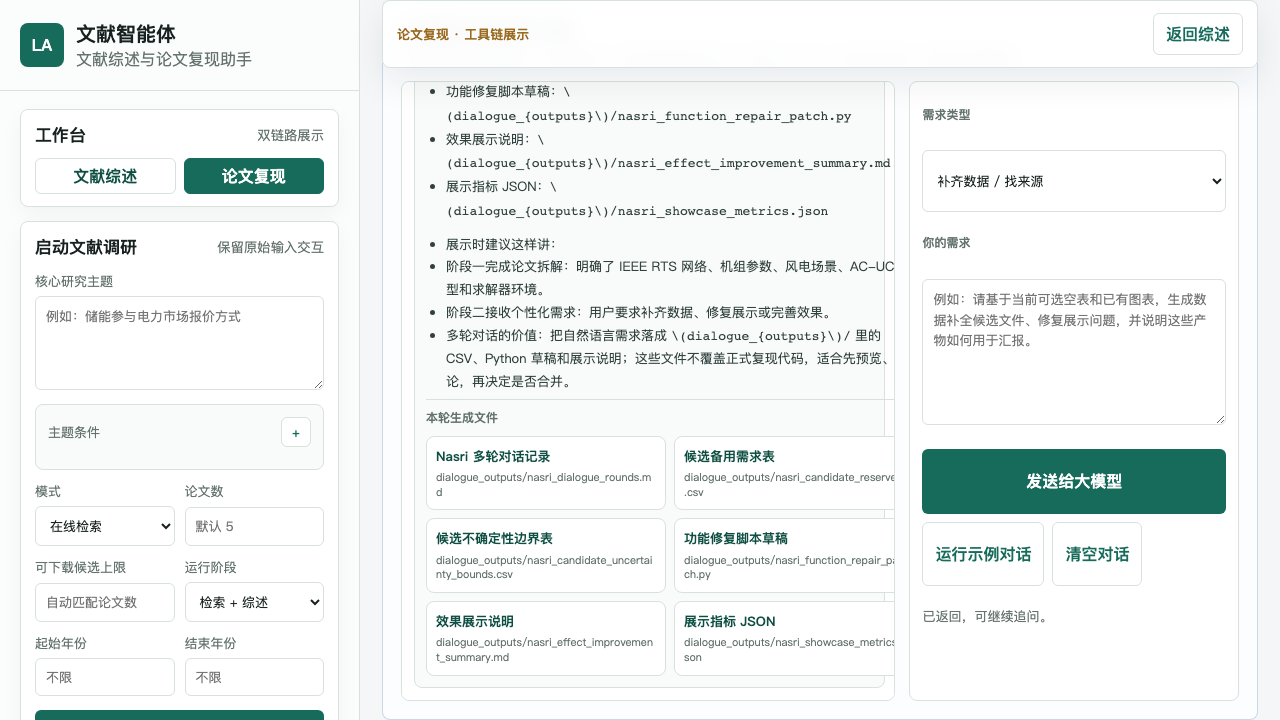
\includegraphics[width=\linewidth]{showcase_dialogue_demo.png}
  \caption{第二阶段多轮对话生成本地产物}
  \label{fig:dialogue-demo}
\end{figure}

\subsection{本轮对话生成了什么}

\begin{longtable}{p{0.22\linewidth}p{0.34\linewidth}p{0.34\linewidth}}
\toprule
\textbf{产物} & \textbf{位置} & \textbf{作用}\\
\midrule
\endhead
多轮对话记录 & \code{dialogue\_outputs/nasri\_dialogue\_rounds.md} & 记录用户意图、模型处理逻辑和每轮落地产物\\
候选备用需求表 & \code{dialogue\_outputs/nasri\_candidate\_reserves.csv} & 基于负荷曲线生成可审查的备用需求候选数据\\
候选不确定性边界表 & \code{dialogue\_outputs/nasri\_candidate\_uncertainty\_bounds.csv} & 将风电 $\pm 20\%$ 和负荷 $\pm 3\%$ 整理成结构化边界\\
功能修复脚本草稿 & \code{dialogue\_outputs/nasri\_function\_repair\_patch.py} & 修复“可选空表被误解成失败”的校验展示问题\\
效果展示说明 & \code{dialogue\_outputs/nasri\_effect\_improvement\_summary.md} & 给出汇报话术和文件用途说明\\
展示指标 JSON & \code{dialogue\_outputs/nasri\_showcase\_metrics.json} & 汇总完整数据表、图表、对话轮数和新增产物\\
\bottomrule
\end{longtable}

\subsection{为什么这体现阶段二的有效性}

\begin{enumerate}
  \item 阶段二把自然语言需求转成了可检查文件。用户不是只得到一段建议，而是得到 CSV、Python 草稿和说明文档。
  \item 阶段二不直接覆盖正式复现代码。所有生成内容先进入 \code{dialogue\_outputs/}，适合预览、讨论和人工确认，确认后再合并到 \code{data/} 或 \code{src/}。
  \item 阶段二能处理个性化问题。同样是 Nasri 论文，用户可以要求补数据、修脚本、解释图表差距或准备展示材料，每次都可以使用当前工作区文件作为上下文继续推进。
\end{enumerate}

\section{结果展示}

结果区已经精简为 4 张关键图，避免 PNG/SVG 重复和 CSV 预览堆叠：

\begin{itemize}
  \item Fig. 3 风电场景重构。
  \item Fig. 4 发电与承诺调度。
  \item Fig. 5 Benders 收敛曲线。
  \item 原文结果与当前实现对比。
\end{itemize}

\begin{figure}[htbp]
  \centering
  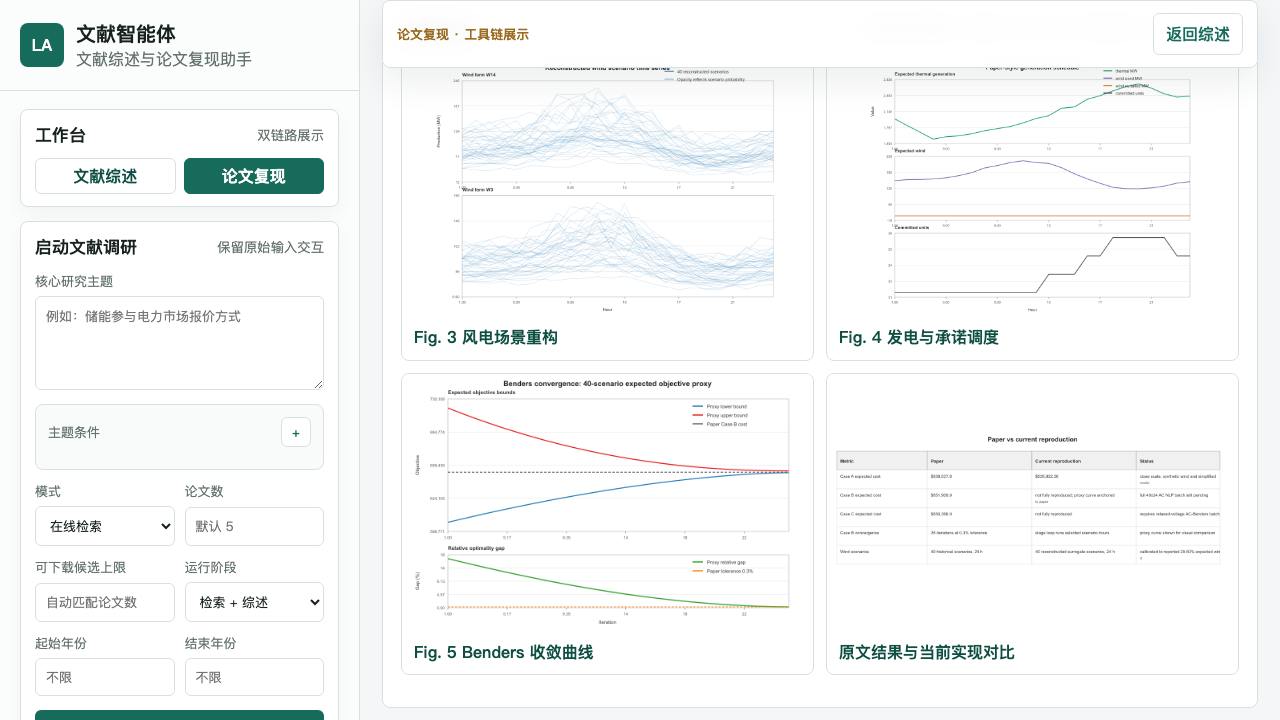
\includegraphics[width=\linewidth]{showcase_clean_results.png}
  \caption{精简后的结果展示区}
  \label{fig:clean-results}
\end{figure}

展示时可以说明：结果区只呈现最适合汇报的图。完整 CSV、SVG 和中间结果仍保留在阶段二文件缓存区，用户可以在需要时打开或交给大模型继续解释。

\section{建议展示话术}

可以按下面顺序讲：

\begin{enumerate}
  \item 先说明阶段一：系统从论文中拆出数据来源、模型结构和环境配置，形成可复现工作流。
  \item 再展示数据来源分层：原文表格、公开 RTS/MATPOWER 和原文图形替代构造，最后统一进入 CSV 数据层。
  \item 然后进入阶段二：用户通过多轮对话提出个性化需求，例如补齐备用需求、生成不确定性边界、修复展示逻辑。
  \item 打开 \code{dialogue\_outputs/} 里的生成文件，强调这些是可审查的本地产物。
  \item 最后展示关键结果图，说明阶段二生成的文件服务于后续数据确认、脚本修复和结果解释。
\end{enumerate}

\textbf{一句话总结：}阶段一解决“论文复现需要什么”，阶段二解决“用户现在想怎么推进”。多轮对话的价值不只是回答问题，而是把问题转成本地可检查、可复用、可合并的工作文件。

\end{document}
